\documentclass[tikz]{standalone}
\usepackage{amsmath}
\usepackage{tikz}

\begin{document}

\begin{figure}[H]
\begin{center}
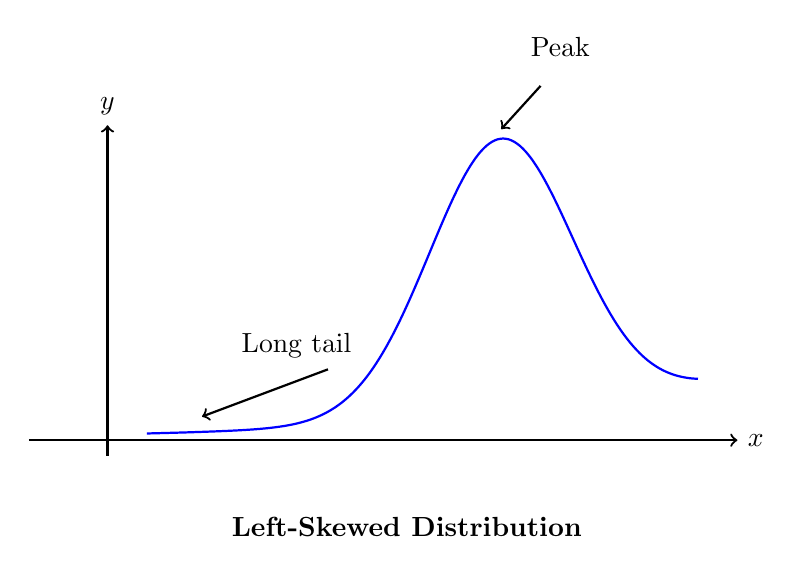
\begin{tikzpicture}
  \draw[thick, ->] (-1,0) -- (8,0) node[right] {$x$};
  \draw[thick, ->] (0,-0.2) -- (0,4) node[above] {$y$};

  \draw[thick, blue, smooth, samples=100, domain=0.5:7.5] 
    plot (\x, {3.5*exp(-0.6*(\x - 5)^2) + 0.6*exp(-0.3*(7 - \x))});
    
  \node at (3.8,-1.1) {\textbf{Left-Skewed Distribution}};
  
  \node at (2.4,1.2) {Long tail};
  \draw[->, thick] (2.8,0.9) -- (1.2,0.3);

  \node at (5.75,5) {Peak};
  \draw[->, thick] (5.5,4.5) -- (5.0,3.95);
\end{tikzpicture}
\end{center}
\caption{An illustration of a left (negative) skewed distribution.}
\end{figure}

\end{document}